\documentclass[conference]{IEEEtran}
\IEEEoverridecommandlockouts
\usepackage{cite}
\usepackage{amsmath,amssymb,amsfonts}
\usepackage{algorithmic}
\usepackage{graphicx}
\usepackage{textcomp}
\usepackage{xcolor}
\usepackage{longtable}
\usepackage{booktabs}
\usepackage{array}
\usepackage{caption}
\usepackage{ragged2e}
\usepackage{url}
\usepackage{svg}
\def\BibTeX{{\rm B\kern-.05em{\sc i\kern-.025em b}\kern-.08em
    T\kern-.1667em\lower.7ex\hbox{E}\kern-.125emX}}


\newcommand{\mfabric}{PQ-Fabric}

\renewcommand{\topfraction}{0.95}
\renewcommand{\bottomfraction}{0.95}
\renewcommand{\textfraction}{0.05}
\renewcommand{\floatpagefraction}{0.85}
\setcounter{topnumber}{3}
\setcounter{bottomnumber}{3}
\setcounter{totalnumber}{6}
\raggedbottom

\begin{document}

\title{A Quantum Threat Model for Hyperledger Fabric: Cryptographic Audit, Risk Prioritisation, and Formal Integration Requirements}

\author{\IEEEauthorblockN{Zara Laila Cheong}
\IEEEauthorblockA{\textit{School of Digital Science} \\
\textit{Universiti Brunei Darussalam}\\
Bandar Seri Begawan, Brunei \\
zaralaila@icloud.com}
\and
\IEEEauthorblockN{Ali Tufail}
\IEEEauthorblockA{\textit{School of Digital Science} \\
\textit{Universiti Brunei Darussalam}\\
Bandar Seri Begawan, Brunei \\
ali.tufail@ubd.edu.bn}
\and
\IEEEauthorblockN{Rosyzie Anna Apong}
\IEEEauthorblockA{\textit{School of Digital Science} \\
\textit{Universiti Brunei Darussalam}\\
Bandar Seri Begawan, Brunei \\
rosyzie.apong@ubd.edu.bn}
}

\maketitle

\begin{abstract}
Cryptographically relevant quantum computers (CRQCs) threaten every system whose security rests on the elliptic curve discrete logarithm problem (ECDLP). Hyperledger Fabric, the dominant enterprise permissioned blockchain, depends uniformly on ECDSA and ECDH over P-256 across its entire transaction lifecycle and identity infrastructure. This paper presents the first component-level quantum vulnerability audit and formal threat model for Hyperledger Fabric. Auditing v2.5.12, we identify twenty-five distinct quantum-vulnerable operations across five lifecycle phases, the Fabric CA and MSP identity subsystems, the gossip protocol, and the key management layer, confirming that the vulnerability is complete and uniform: every public-key operation is simultaneously broken by Shor's algorithm. From this inventory we derive five formal threat scenarios with explicit adversarial assumptions and prioritise them in a severity--exploitability risk matrix. We show that the append-only ledger permanently amplifies the harvest-now-decrypt-later (HNDL) threat, and we adapt Mosca's inequality to this setting across five deployment scenarios. The analysis identifies root-CA self-signing and orderer block-signing as the highest-priority migration targets and exposes a partial migration vulnerability in which post-quantum transaction signing gives no protection while the CA remains classical. We conclude with eight formal integration requirements, traceable to the identified threats, that specify a quantum-resistant Fabric architecture, including the requirement that the live CA itself issue post-quantum certificates at runtime.
\end{abstract}

\begin{IEEEkeywords}post-quantum cryptography, Hyperledger Fabric, permissioned blockchain, quantum threat model, harvest-now-decrypt-later
\end{IEEEkeywords}

\section{Introduction}
\label{sec:tm_intro}
Quantum computing introduces a cryptographic threat fundamentally different
from classical vulnerabilities. While classical attacks exploit implementation
errors or weak parameters, Shor's algorithm renders algorithms based on the
discrete logarithm or integer factorisation problem insecure on a
cryptographically relevant quantum computer (CRQC)~\cite{shor1994}. Once such
a device exists, migration to post-quantum cryptography (PQC) becomes the only
effective defence.

Hyperledger Fabric, widely deployed across finance, healthcare, supply chain,
and government~\cite{androulaki2018}, relies on ECDSA and ECDH P-256
throughout its transaction lifecycle and identity infrastructure. Because both
depend on the ECDLP, a CRQC could recover private keys, forge signatures, and
decrypt recorded TLS sessions.

The harvest-now-decrypt-later (HNDL) threat is especially severe in
blockchains. Fabric's immutable ledger permanently stores transaction
signatures, block-header signatures, and certificate chains, leaving
historical cryptographic material vulnerable even after migration. For
long-lived data, the threat therefore applies to the entire ledger history,
not only future records.
Despite growing recognition of quantum threats to
blockchains~\cite{fernandez2020, yang2024survey}, no prior work has produced a
component-level quantum vulnerability audit for Fabric, and existing PQC
integration proposals lack formal threat
analysis~\cite{holcomb2021, campbell2019, hu2025prototype, razdan2025postquantum}. This paper makes the following contributions:
\begin{itemize}
    \item The first component-level quantum vulnerability audit of Hyperledger Fabric is conducted, identifying twenty-five vulnerable operations across the transaction lifecycle and identity infrastructure.
    \item Five formal threat scenarios are defined, with explicit mapping to the HNDL (Harvest Now, Decrypt Later) dimensions.
    \item A risk prioritization matrix is proposed to facilitate the assessment and mitigation of identified vulnerabilities.
    \item A Mosca inequality analysis is performed to evaluate the urgency of quantum threats for representative Hyperledger Fabric deployments.
    \item Eight integration requirements are outlined to define a quantum-resistant architecture for Hyperledger Fabric.
\end{itemize}
Collectively, these contributions bridge the gap between theoretical quantum risk and practical engineering, providing the first actionable blueprint for securing Hyperledger Fabric against both immediate HNDL threats and future cryptanalytic breakthroughs.

\section{Methodology}
\label{sec:tm_method}
This section defines the scope, target system, and analytical framework of the audit, and sets out the four-stage process by which each cryptographic operation is enumerated, mapped, classified, and rated. It also establishes the severity rubric used throughout the paper, calibrated on the scope of compromise rather than the reversibility of the consequence.


\subsection{Scope and Target System}
The audit targets Hyperledger Fabric v2.5.12 and covers the full transaction
lifecycle, including the client SDK, endorsing peers, Raft ordering service,
Fabric CA, and MSP. Sources include Fabric documentation, the Blockchain Cryptographic Service Provider (BCCSP) interface,
and configuration schemas.
Hash functions and AES-256 are excluded because, although affected by
Grover's algorithm~\cite{grover1996}, they retain acceptable post-quantum
security under current NIST guidance~\cite{nist_sp80057}. The audit therefore
focuses on asymmetric operations vulnerable to Shor's algorithm.

\subsection{Analytical Framework}
Existing frameworks such as CVE, OWASP Cryptographic Failures, and
NIST SP~800-57~\cite{nist_sp80057} do not address the structural quantum
vulnerability of correctly implemented ECDSA systems. The analysis therefore
combines structured threat modelling~\cite{shostack2014, stride2004} with
quantum-specific classification informed by NIST PQC
literature~\cite{nist_ir8105, bernstein2017pqc}.

\subsection{Four-Stage Audit Process and Severity Rubric}
\label{sec:tm_severity}
The audit, summarised in Figure~\ref{fig:ch4_methodology}, proceeds in
four stages: (1) enumerates lifecycle cryptographic operations;
(2) maps each to its algorithm and key type; (3) classifies operations
as Shor-threatened or Grover-affected; and (4) assesses severity and
exploitability.
Severity is based on compromise scope. \textbf{Critical} applies to compromise
of network-wide trust or trust anchors; \textbf{High} to transaction or
identity-level compromise; \textbf{Medium} to confidentiality breaches such as
TLS decryption; and \textbf{Low} to limited information exposure, though no
operations in this audit fall into that category.

\begin{figure*}
    \centering
    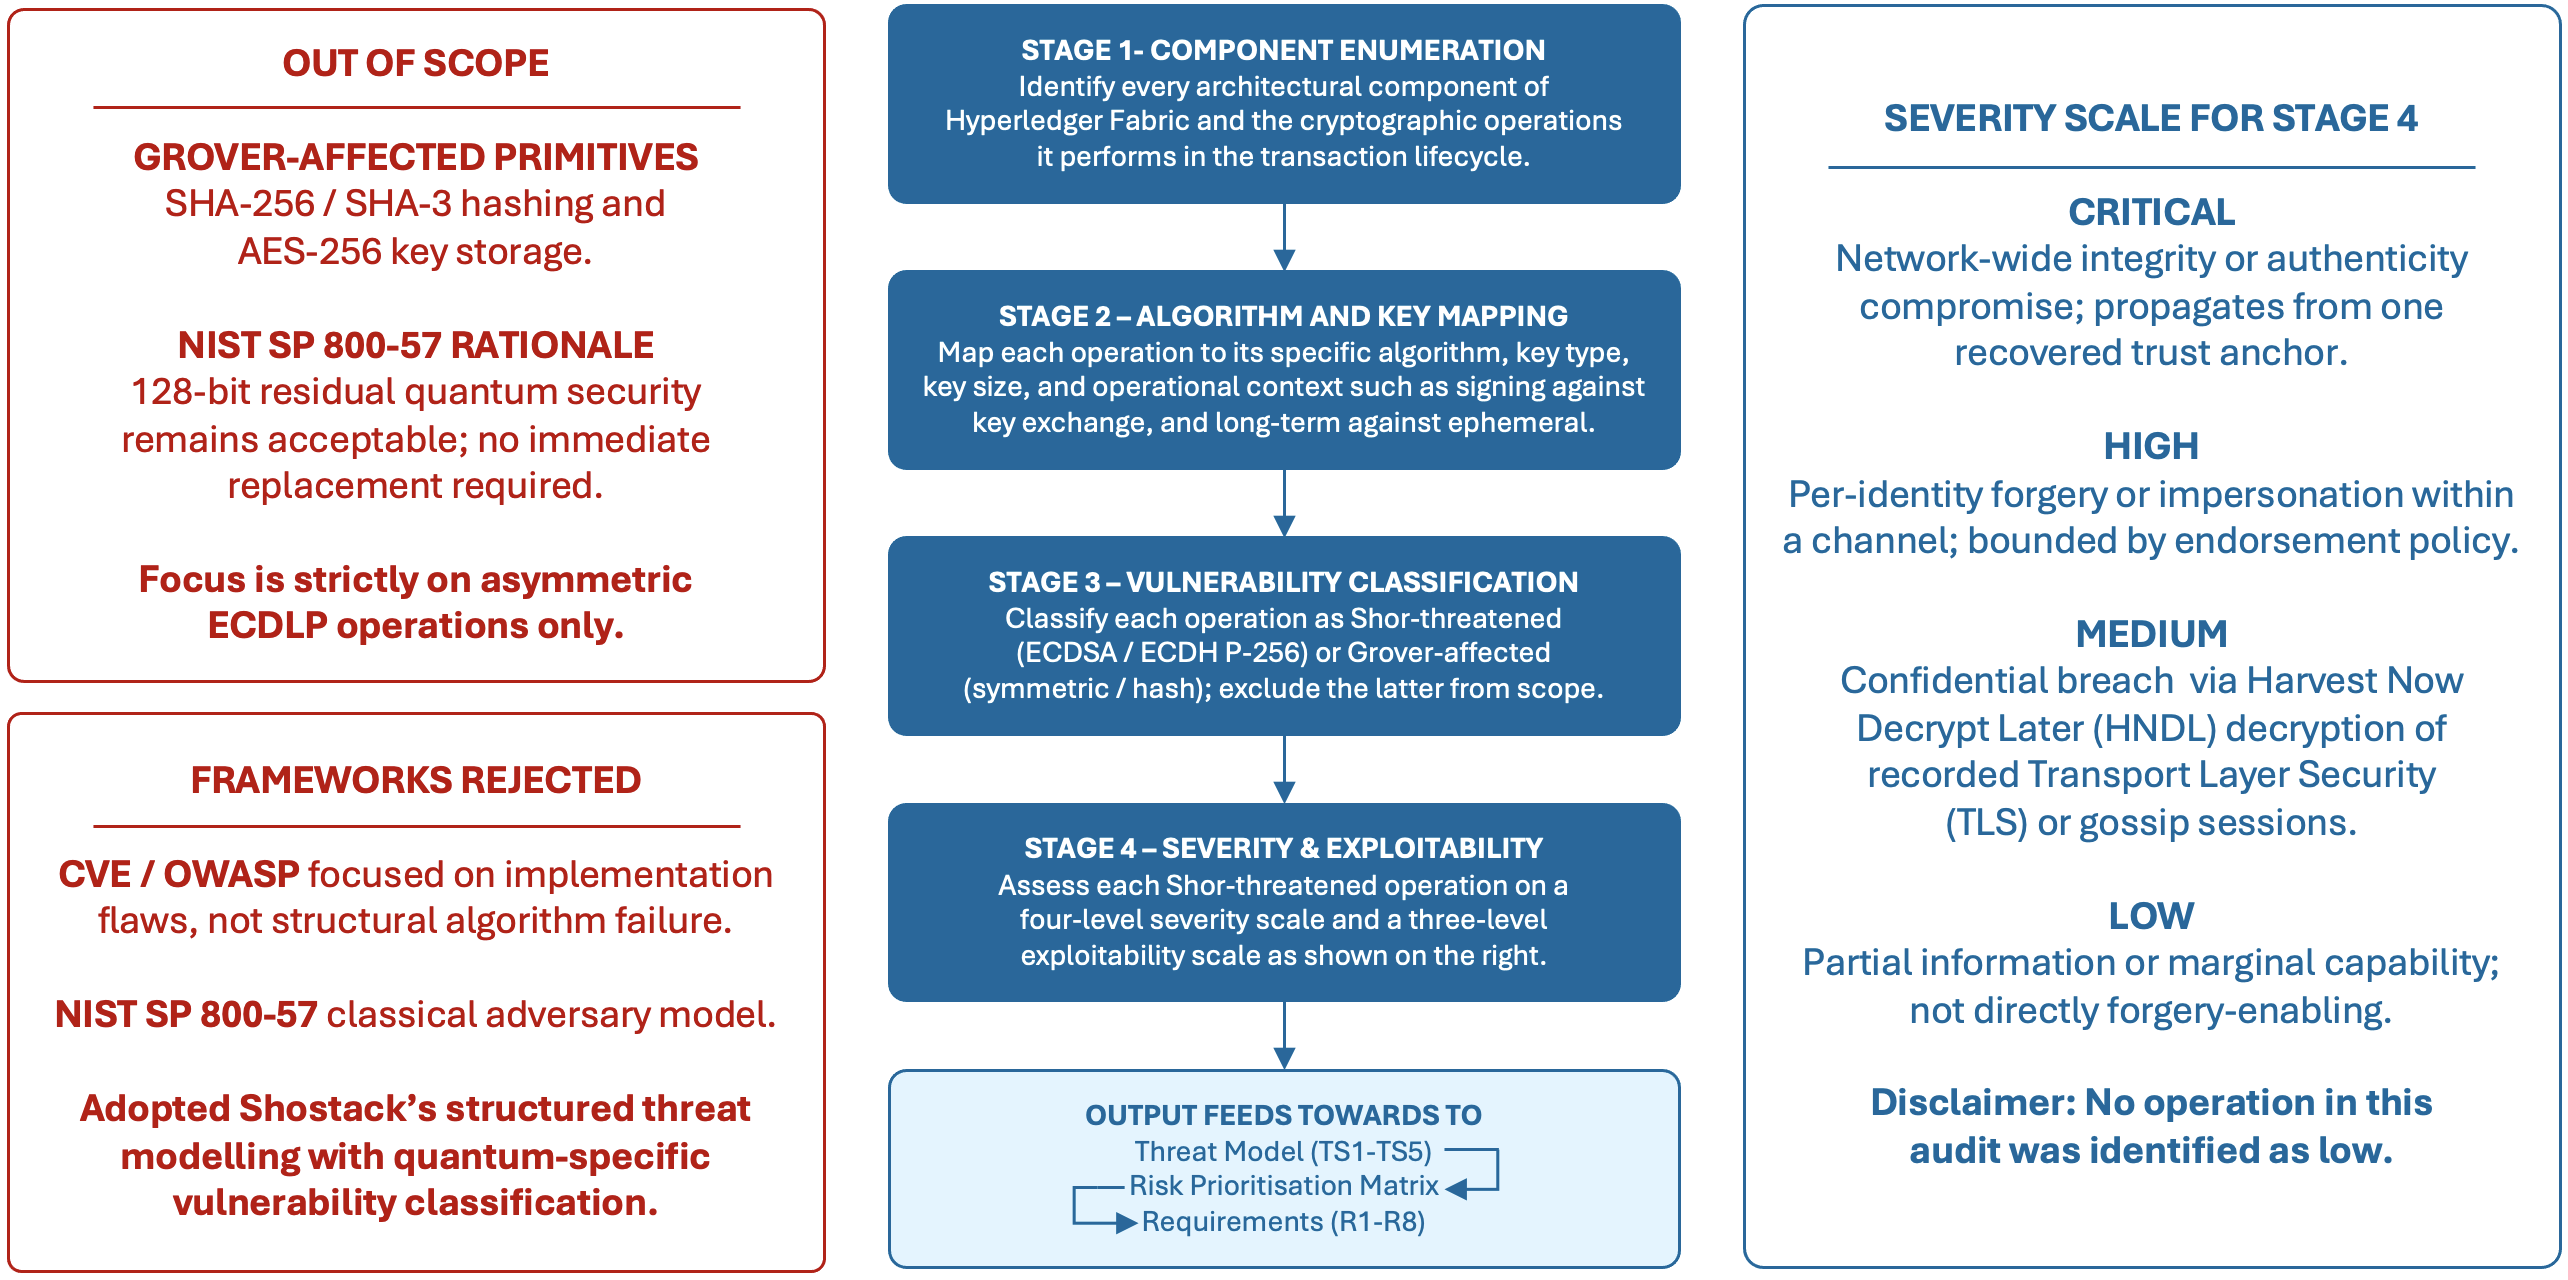
\includegraphics[width=\linewidth]{figures/fig_auditability_methodology.png}
    \caption{Hyperledger Fabric Quantum Vulnerability Audit Methodology}
    \label{fig:ch4_methodology}
\end{figure*}

\section{Cryptographic Inventory}
\label{sec:tm_inventory}
This section applies the audit process to Hyperledger Fabric v2.5.12, enumerating all identified 25 quantum-vulnerable operations across the five transaction lifecycle phases, the identity infrastructure, the gossip protocol, and the key management layer. It establishes the uniform ECDLP dependence of the platform and analyses the performance significance of signature verification at scale.

\subsection{Uniform ECDLP Dependence}
The audit reveals complete and uniform dependence on the ECDLP across all
public-key functions in the standard lifecycle. Every digital signature uses
ECDSA P-256; every session-key exchange uses ECDH P-256. There is no
cryptographic diversity: all asymmetric guarantees rest on the same hardness
assumption and are simultaneously eliminated by Shor's algorithm. The audit
identifies twenty-five distinct quantum-vulnerable operations across five
lifecycle phases, two identity subsystems, the gossip protocol, and the key
management layer (Table~\ref{tab:crypto_inventory}).

Given an elliptic curve $E$ over $\mathbb{F}_p$, a base point
$G \in E(\mathbb{F}_p)$ of prime order $n$, and $Q \in E(\mathbb{F}_p)$, the
ECDLP is to find the unique $k \in \{1,\ldots,n-1\}$ with

\begin{equation}
Q = kG.
\label{eq:ecdlp}
\end{equation}

The best-known classical algorithm, Pollard's rho, requires $O(\sqrt{n})$ group
operations; for P-256, $n \approx 2^{256}$, giving $\approx 2^{128}$ operations.
Shor's algorithm reduces this to $O((\log n)^3)$ quantum
gates~\cite{shor1994}:

\begin{equation}
T_{\mathrm{classical}} = O\!\left(\sqrt{n}\right),
\qquad
T_{\mathrm{quantum}} = O\!\left((\log n)^3\right).
\label{eq:complexity}
\end{equation}

Defining the security level $\lambda$ as the binary logarithm of the best-known
attack cost, the classical-to-quantum transition for ECDSA P-256 is

\begin{equation}
\lambda_{\mathrm{classical}} \approx 128\text{ bits},
\qquad
\lambda_{\mathrm{quantum}} = 0.
\label{eq:security_bits}
\end{equation}

Equation~(\ref{eq:security_bits}) establishes that no implementation or
parameter change restores security once Shor's algorithm is executable at the
target key size --- the property distinguishing the quantum vulnerability from
all classical vulnerabilities.

\subsection{Lifecycle Operations (Op-01--Op-16)}

\textbf{Phase~1 - Proposal/client signing.}
Op-01 (client proposal signing, ECDSA) authenticates client actions; forgery
enables arbitrary proposals. High. Op-02 (client$\rightarrow$peer TLS, ECDH)
allows retroactive decryption of recorded traffic. Medium.

\textbf{Phase~2 - Endorsement.}
Op-03 (proposal signature verification) protects transaction processing. High.
Op-04 (X.509 chain validation) establishes identity authenticity; forged
certificates enable channel-wide impersonation. Critical. Op-05 (endorsement
signing) binds peers to transaction results; forgery enables fake endorsements.
High. Op-06 (peer TLS) exposes long-term TLS keys. Medium.

\textbf{Phase~3 - Assembly/submission.}
Op-07 (envelope signing) authenticates endorsed transactions. High. Op-08
(client$\rightarrow$orderer TLS) exposes pending transactions before
commitment. Medium.

\textbf{Phase~4 - Ordering/block signing.}
Op-09 (envelope verification) is the final authentication step before ordering.
High. Op-10 (block-header signing) is the most critical operation, since forged
signatures enable irreversible insertion of fraudulent blocks. Critical.
Op-11 (orderer$\rightarrow$peer TLS) protects block delivery. Medium. Op-12
(Raft mutual TLS authentication) protects consensus integrity. High. Op-13
(Raft TLS key exchange) exposes consensus traffic and may enable manipulation
when combined with Op-12. High.

\textbf{Phase~5 - Committing-peer validation.}
Op-14 (endorsement re-verification) is the most performance-sensitive operation
under PQC and creates permanent HNDL targets. High. Op-15 (block-header
verification) is the final integrity check before commit. Critical. Op-16
(certificate re-validation) is the final defence against fraudulent
certificates before permanent ledger commitment. Critical.

\subsection{Identity Infrastructure, Gossip, and Key Management (Op-17--Op-25)}
\textbf{Fabric CA.}
Op-17 (root CA self-signing) is the network trust anchor; compromise enables
arbitrary certificate issuance. Critical. Op-18 (intermediate CA signing)
extends compromise through the CA hierarchy. Critical. Op-19 (end-entity
issuance) affects identities under the compromised CA. High. Op-20 (CA
enrolment TLS) exposes participant identity data. Medium.

\textbf{MSP.}
Op-21 (MSP validation) accepts certificates from a compromised root CA.
Critical. Op-22 (channel configuration signing) forgery enables arbitrary
policy and organisation changes. Critical.

\textbf{Gossip and key management.}
Op-23 (gossip signing) can disrupt peer synchronisation. Medium. Op-24
(gossip TLS) exposes uncommitted data. Medium. Op-25 (BCCSP keypair generation)
requires full identity regeneration during PQC migration. High.

\subsection{Signature Verification at Scale}
\label{sec:tm_scale}
Op-14 (endorsement re-verification) is executed by every committing peer for every transaction, processing thousands of verifications per second at moderate throughput. The performance impact of Post-Quantum Cryptography (PQC) is amplified beyond verification time: larger signatures increase block sizes, slowing gossip propagation and reducing sustainable throughput. Since each transaction carries multiple endorsements with full certificate chains, replacing compact ECDSA signatures with significantly larger PQC alternatives severely impacts storage and network bandwidth. Consequently, \emph{signature output size is a more critical performance determinant than signing speed} for blockchain PQC migration.

Let $T_b$ be transactions per block, $\bar{e}$ the average endorsers per
transaction, $|\sigma_{\mathrm{alg}}|$ the signature size, and
$|\mathit{cert}_{\mathrm{alg}}|$ the certificate-chain size. The Op-14
cryptographic payload per block is

\begin{equation}
B_{\sigma} = T_b \cdot \bar{e} \cdot
\bigl(|\sigma_{\mathrm{alg}}| + |\mathit{cert}_{\mathrm{alg}}|\bigr).
\label{eq:block_payload}
\end{equation}

With $\tau(|\sigma|)$ the per-signature verification time and
$C_{\mathrm{val}}$ a peer's validation capacity, the maximum sustainable
throughput is bounded by

\begin{equation}
\Gamma_{\max} \;\leq\; \frac{C_{\mathrm{val}}}{T_b \cdot \bar{e} \cdot
\tau(|\sigma_{\mathrm{alg}}|)}.
\label{eq:tps_bound}
\end{equation}

A smaller $|\sigma_{\mathrm{alg}}|$ reduces $B_{\sigma}$
in~(\ref{eq:block_payload}), decreasing propagation latency and relaxing the
bound in~(\ref{eq:tps_bound}) even when $\tau(|\sigma|)$ is higher --- motivating
FN-DSA-512 for throughput-sensitive deployments despite its slower signing
relative to ML-DSA-44.

\subsection{Complete Inventory}
Figure~\ref{fig:crypto_inventory} maps all twenty-five quantum-vulnerable
operations across eight component groups: the five transaction-lifecycle
phases, the Fabric CA/MSP identity infrastructure, the gossip protocol, and
the key management layer. Fabric CA/MSP contains the highest
concentration of Critical operations, with Op-17 forming the primary TS1 attack
surface because the root CA key remains exposed in the genesis block. ECDH-based
TLS operations (Op-02, 06, 08, 11, 13, 20, 24) appear throughout the lifecycle,
showing that HNDL affects all communication layers.

%--------- Trying t revise the below figure but still ------------
\begin{figure}[tbp]
\centering
\includesvg[inkscapelatex=false,width=\textwidth,width=3.5in,keepaspectratio]{figures/fig_crypto_inventory}
\caption{Cryptographic inventory of Hyperledger Fabric v2.5.12, showing all twenty-five quantum-vulnerable operations.}
\label{fig:crypto_inventory}
\end{figure}

%--------------------------------------
Figure~\ref{fig:threat_model_overview} summarises the component-level threat
model. Red components contain Critical operations, while the dashed red overlay
marks the TS1 attack surface. The dashed blue layer represents TLS-based TS4
exposure across inter-component communication.

\begin{figure}[tbp]
\centering
\includesvg[inkscapelatex=false,width=\textwidth,width=3.5in,keepaspectratio]{figures/fig_threat_model}
\caption{Quantum vulnerability overview for Hyperledger Fabric v2.5.12, color-coded by severity across six components.}
\label{fig:threat_model_overview}
\end{figure}

Table~\ref{tab:crypto_inventory} lists all twenty-five operations with algorithm
and severity. The vulnerability is complete (every public-key operation) and
uniform (every operation ECDLP-based). The distribution is eight critical, ten
high,,  and seven medium, with critical operations concentrated in the certificate
infrastructure, the block signing/verification path, and MSP validation 
confirming that the integrity backbone is most directly threatened.

\begin{table}[t]
\centering
\caption{Complete cryptographic inventory of Hyperledger Fabric v2.5.12. All twenty-five operations use ECDLP-based mathematics and are threatened by Shor's algorithm.}
\label{tab:crypto_inventory}
\footnotesize
\setlength{\tabcolsep}{4pt}
\begin{tabular}{@{}p{0.5cm}>{\raggedright\arraybackslash}p{4.0cm}%
  >{\raggedright\arraybackslash}p{2.0cm}c@{}}
\toprule
\textbf{Op} & \textbf{Operation} & \textbf{Algorithm} &
\textbf{Severity} \\
\midrule
\multicolumn{4}{@{}l}{\textbf{Phase 1 : Transaction Proposal}} \\[1pt]
01 & Client transaction proposal signing   & ECDSA P-256 & High \\
02 & Client TLS handshake to peer          & ECDH P-256  & Medium \\[3pt]
\multicolumn{4}{@{}l}{\textbf{Phase 2 : Peer Endorsement}} \\[1pt]
03 & Client signature verification at peer & ECDSA P-256 & High \\
04 & X.509 certificate chain validation    & ECDSA P-256 & Critical \\
05 & Chaincode execution result signing    & ECDSA P-256 & High \\
06 & Peer TLS inbound/outbound sessions    & ECDH P-256  & Medium \\[3pt]
\multicolumn{4}{@{}l}{\textbf{Phase 3 : Transaction Assembly}} \\[1pt]
07 & Client transaction envelope signing   & ECDSA P-256 & High \\
08 & Client-to-orderer TLS session         & ECDH P-256  & Medium \\[3pt]
\multicolumn{4}{@{}l}{\textbf{Phase 4 : Ordering Service}} \\[1pt]
09 & Envelope sig.\ verification at orderer & ECDSA P-256 & High \\
10 & Block header signing by orderer       & ECDSA P-256 & Critical \\
11 & Orderer-to-peer TLS (block broadcast) & ECDH P-256  & Medium \\
12 & Raft inter-orderer mutual TLS auth    & ECDSA P-256 & High \\
13 & Raft inter-orderer TLS key exchange   & ECDH P-256  & High \\[3pt]
\multicolumn{4}{@{}l}{\textbf{Phase 5 : Committing Peer Validation}} \\[1pt]
14 & Endorsement sig.\ re-verification     & ECDSA P-256 & High \\
15 & Block header signature verification   & ECDSA P-256 & Critical \\
16 & Certificate chain re-validation       & ECDSA P-256 & Critical \\[3pt]
\multicolumn{4}{@{}l}{\textbf{Fabric CA: Certificate Infrastructure}} \\[1pt]
17 & Root CA certificate self-signing      & ECDSA P-256 & Critical \\
18 & Intermediate CA certificate signing   & ECDSA P-256 & Critical \\
19 & End-entity certificate issuance       & ECDSA P-256 & High \\
20 & Fabric CA TLS session                 & ECDH P-256  & Medium \\[3pt]
\multicolumn{4}{@{}l}{\textbf{MSP: Identity Validation}} \\[1pt]
21 & MSP certificate chain validation      & ECDSA P-256 & Critical \\
22 & MSP channel configuration signing     & ECDSA P-256 & Critical \\[3pt]
\multicolumn{4}{@{}l}{\textbf{Gossip Protocol}} \\[1pt]
23 & Gossip message signing                & ECDSA P-256 & Medium \\
24 & Gossip TLS sessions                   & ECDH P-256  & Medium \\[3pt]
\multicolumn{4}{@{}l}{\textbf{Key Management}} \\[1pt]
25 & BCCSP keypair generation              & ECDSA P-256 & High \\
\bottomrule
\end{tabular}
\end{table}

\section{Quantum Threat Model}
\label{sec:tm_threats}
This section translates the inventory into five formal threat scenarios, each with explicit adversarial capability assumptions, impact assessment, and a harvest-now-decrypt-later dimension specific to the immutable ledger. The scenarios range from network-wide certificate forgery to confidentiality-only TLS decryption.

\subsection{Adversarial Capability Model}
The adversary possesses a CRQC capable of executing Shor's algorithm against
P-256; breaking ECDSA P-256 requires approximately 2{,}330 logical qubits with
error correction~\cite{roetteler2017}, with similar estimates for
RSA-2048~\cite{gidney2021}. Although such devices do not yet exist, HNDL makes
them relevant for long-term data~\cite{mosca2018}. Classically, the adversary
can observe network traffic and access public ledger, configuration, and
historical transaction data without privileged access. Physical node compromise
and classical Raft-majority corruption are excluded.


\subsection{TS1: Identity Impersonation via Certificate Forgery}
\textit{Severity: Critical. Exploitability: High. Priority: P1.}
TS1 targets the root CA certificate in the genesis block. Using publicly available MSP configurations and a CRQC, an adversary applies Shor's algorithm to recover the ECDSA root private key and issue valid certificates for arbitrary identities and roles. Forged administrator signatures also enable fraudulent channel updates (Op-22). Because trust propagates through the CA hierarchy, compromising the root key compromises all derived certificates. The HNDL risk is permanent since the root key remains embedded on-chain from genesis. \emph{Affected operations: Op-04, Op-16, Op-17, Op-18, Op-19, Op-21, Op-22.}

\subsection{TS2: Transaction Signature Forgery}
\textit{Severity: High. Exploitability: High. Priority: P2.}
TS2 targets ECDSA signatures on proposals, endorsements, and transaction envelopes. Since transaction records expose verification keys, any ledger reader can harvest them. After recovering a private key with Shor's algorithm, the adversary can sign fraudulent transactions or endorsements as the compromised identity, including bypassing multi-organisation endorsement policies. The HNDL threat persists permanently because historical ledger data cannot be removed. \emph{Affected operations: Op-01, Op-03, Op-05, Op-07, Op-09, Op-14.}

\subsection{TS3: Block Integrity Compromise via Orderer Key Recovery}
\textit{Severity: Critical. Exploitability: High. Priority: P1.}
TS3 targets orderer block-signing keys exposed in block headers. Recovering an orderer private key enables valid signatures on fraudulent blocks, allowing insertion, reordering, or suppression of transactions. Since committed blocks become permanently embedded in the ledger hash chain, integrity compromise is effectively irreversible. Compromising Raft inter-orderer authentication (Op-12/Op-13) further enables consensus manipulation through MITM attacks. \emph{Affected operations: Op-10, Op-12, Op-13, Op-15.}

\subsection{TS4: TLS Session Decryption via HNDL}
\textit{Severity: Medium. Exploitability: Medium. Priority: P3.}
TS4 targets ECDH P-256 used in TLS sessions. An adversary records encrypted traffic and later uses Shor's algorithm to recover session keys from captured handshakes, decrypting historical communications. Exposed data may include proposals, endorsements, block contents, and administrative traffic. Ephemeral ECDH provides no effective forward secrecy against a quantum adversary. \emph{Affected operations: Op-02, Op-06, Op-08, Op-11, Op-13, Op-20, Op-24.}


\subsection{TS5: Gossip Protocol Manipulation}
\textit{Severity: Medium. Exploitability: Low. Priority: P4.}
TS5 recovers a peer's gossip signing key from observable discovery messages and
injects fraudulent gossip, or decrypts recorded gossip TLS. Two impacts arise:
state-synchronisation manipulation (false block announcements, unnecessary state
transfers, incorrect ledger height, or restoring a recovering peer from a
fraudulent state) and transaction-content exposure (advance knowledge of
propagating block content, constituting material non-public information in
financial networks). Exploitability is Low because TS5 requires a network
position to observe or inject gossip, unlike the P1/P2 threats executable by any
ledger reader. \emph{Affected operations: Op-23, Op-24.}

Figure~\ref{fig:threat_attack_paths} maps each scenario to its entry point
(downward arrow) and impacted components (filled circles). TS1 and TS3 originate
from key material permanently accessible on the ledger (genesis-block CA
certificate; orderer key in block headers); TS2 originates at the BCCSP signing
layer; TS4/TS5 require active network observation and are rated Medium.

\begin{figure}[t]
\centering
\includesvg[inkscapelatex=false,width=\linewidth,height=2.4in,keepaspectratio]{figures/fig_threat_attack_paths}
\caption{Threat scenario attack paths mapped to Fabric components: entry points and impacted components.}
\label{fig:threat_attack_paths}
\end{figure}

\section{Risk Prioritisation}
\label{sec:tm_risk}
This section orders the five threat scenarios by severity and exploitability in a risk matrix, derives the resulting migration priorities, and formalises the analysis with a composite risk score. It also exposes the partial migration vulnerability, in which post-quantum transaction signing provides no protection while the certificate authority remains classical.

\subsection{Risk Matrix}
Table~\ref{tab:risk_matrix} assesses each scenario by severity and
exploitability, determining migration priority. TS1 and TS3 share the joint
highest priority (Critical, High); TS2 is second (High, High); TS4 and TS5 are
lower, constrained by network-observation requirements more demanding than
passive ledger reading.

\begin{table}[t]
\centering
\caption{Risk prioritization matrix for the five quantum threat scenarios identified in the Hyperledger Fabric v2.5.12 audit.}
\label{tab:risk_matrix}
\setlength{\tabcolsep}{3pt}
\footnotesize
\begin{tabular}{@{}>{\raggedright\arraybackslash}p{0.7cm}>{\raggedright\arraybackslash}p{5cm}cc@{}}
\toprule
\textbf{Prio.} & \textbf{Scenario} & \textbf{Severity} &
\textbf{Exploit} \\
\midrule
P1 & TS1: Identity Impersonation & Critical & High \\
P1 & TS3: Block Integrity Compromise & Critical & High \\
P2 & TS2: Tx Signature Forgery & High & High \\
P3 & TS4: TLS Session Decryption & Medium & Medium \\
P4 & TS5: Gossip Manipulation & Medium & Low \\
\bottomrule
\end{tabular}
\end{table}

Three architectural conclusions follow. First, the CA infrastructure and the
block-signing path share top priority and must be addressed simultaneously: both
are accessible to any passive ledger observer, and no measure short of replacing
both with PQC addresses the P1 threats. Second, peer endorsement and client
signing share second priority --- more limited in scope but equally exploitable,
since signatures and keys appear in every historical record. Third, TLS and gossip
occupy lower priority only because exploitation requires network observation; they
remain in the requirements because complete quantum resistance requires the full
attack surface, and HNDL on TLS requires only past observation.

\subsection{Quantitative Risk Synthesis}
\label{sec:tm_risk_quant}

Mapping severity to $s_i \in \{1,2,3\}$ (M/H/C) and exploitability to
$e_i \in \{1,2,3\}$ (L/M/H), the composite score is

\begin{equation}
\rho_i = s_i \cdot e_i.
\label{eq:risk_score}
\end{equation}

TS1 and TS3 yield $\rho = 9$ (P1, maximum); TS2 yields $6$ (P2); TS4 yields $2$
(P3); TS5 yields $1$ (P4). No measure beneath the cryptographic layer can reduce
$s_i$ or $e_i$ for TS1/TS3, as their exploitability derives from immutable ledger
content. Defining the coverage relation
$\Phi \subseteq \{R_1,\ldots,R_8\}\times\{\mathrm{TS1},\ldots,\mathrm{TS5}\}$
with $(R_k,\mathrm{TS}_j)\in\Phi$ iff $R_k$ addresses $\mathrm{TS}_j$, the
requirement set is complete iff

\begin{equation}
\forall\, j \in \{1,\ldots,5\},\;\;
\exists\, k \in \{1,\ldots,8\} \;:\; (R_k,\,\mathrm{TS}_j) \in \Phi.
\label{eq:req_coverage}
\end{equation}

Table~\ref{tab:req_traceability} confirms~(\ref{eq:req_coverage}) holds (TS1 by
$R_3$, TS2/TS3 by $R_1$, TS4/TS5 by $R_2$); completeness is bounded by the scope
of the threat enumeration. Finally, with $\Gamma(t)$ the throughput, $\bar{k}$
the mean new ECDSA keys per transaction, and $\mathbb{1}[t<t_m]$ the
pre-migration indicator, the harvest set grows at

\begin{equation}
\frac{d\,|\mathcal{H}|}{dt}(t) = \Gamma(t)\cdot\bar{k}\cdot\mathbb{1}[t<t_m],
\label{eq:hndl_rate}
\end{equation}

so total accumulated exposure from genesis $t_0$ to evaluation
$t_{\mathrm{eval}}$ is

\begin{equation}
|\mathcal{H}(t_{\mathrm{eval}})| =
\int_{t_0}^{\min(t_m,\,t_{\mathrm{eval}})} \Gamma(t)\,\bar{k}\;\mathrm{d}t
\;\approx\; \bar{\Gamma}\,\bar{k}\,(t_{\mathrm{eval}} - t_0).
\label{eq:hndl_total}
\end{equation}

Equation~(\ref{eq:hndl_total}) makes precise the governance conclusion: every day
under ECDSA P-256 permanently enlarges the harvest set by
$\approx \bar{\Gamma}\cdot\bar{k}\cdot 86{,}400$ keys.

\subsection{The Partial Migration Vulnerability}
\label{sec:tm_partial}

A critical insight is the structural interdependence between the CA layer and
the BCCSP signing layer. If an operator deploys PQC signing at the BCCSP layer
without migrating the certificate infrastructure, the CA public keys in the
channel configuration remain ECDSA. A quantum adversary who recovers the CA
private key issues fraudulent \emph{post-quantum} certificates accepted as
legitimate by any PQC-capable MSP --- the quantum resistance of the signing
layer is completely neutralised by the classical vulnerability of the
certificate layer.

Figure~\ref{fig:partial_migration} contrasts partial migration (left, red=vulnerable) with full compliance (right, teal=secure). In the left panel, although BCCSP/MSP are migrated, the legacy ECDSA CA key in the genesis block allows an attacker to use Shor’s algorithm to forge valid post-quantum certificates, which the MSP inadvertently accepts. This demonstrates that migrating signing algorithms alone is insufficient if the CA remains classical. In the right panel, satisfying R3 by issuing post-quantum CA keys eliminates the harvestable ECDSA material, thereby closing TS1. Thus, R3 is strictly required; deferring CA migration leaves the system vulnerable regardless of BCCSP upgrades.

\begin{figure}[tbp]
\centering
\includesvg[inkscapelatex=false,width=\textwidth,width=3.5in,keepaspectratio]{figures/fig_partial_migration}
\caption{Partial migration vulnerability: TS1 remains fully exploitable when only the BCCSP layer is migrated.}
\label{fig:partial_migration}
\end{figure}

\section{Quantum Attack Timeline Analysis}
\label{sec:tm_mosca}
This section establishes the urgency of migration by relating the security lifetime of protected data to the projected CRQC emergence date and the migration lead time. It applies Mosca's inequality across five representative Fabric deployment scenarios and derives a blockchain-corrected formulation that accounts for the permanent harvest exposure of historical ledger records.

\subsection{Mosca's Inequality}
Urgency requires a temporal analysis relating data security lifetime to the CRQC
emergence date and migration lead time. Mosca's inequality states that if
$X+Y>Z$ migration must begin immediately, where $X$ is years until a CRQC, $Y$ is
migration duration, and $Z$ is the required data security
lifetime~\cite{mosca2018}:

\begin{equation}
X + Y > Z \;\Longrightarrow\; \text{PQC migration must begin immediately.}
\label{eq:mosca}
\end{equation}

Anchored to a 2026 planning base, the optimistic estimate places $X=7$ years
(CRQC $\approx$2033), informed by Mosca's assessment of a one-in-two chance by
2031~\cite{mosca2018}; the pessimistic estimate places $X=15$ years
($\approx$2041). Migration time $Y$ for an enterprise Fabric network is estimated
at 2--3 years, accounting for a production-quality PQC release,
certificate-infrastructure renewal for all identities, staged multi-organisation
rollout, and operational/regulatory validation --- consistent with major
financial-sector PQC planning.

\subsection{Application to Fabric Deployment Scenarios}

Table~\ref{tab:mosca} evaluates the inequality across five scenarios under both
timelines. Three of five satisfy $X+Y>Z$ under both estimates, indicating
immediate action regardless of CRQC timing: healthcare (30+ year retention),
financial settlement (20+ years), and government procurement (25+ years). Supply
chain is \textit{Borderline/Immediate}: records span $Z\!\approx\!5$ (inventory)
to $Z\!\approx\!10$ (regulated provenance); under the optimistic timeline
($X+Y=10$) the inequality holds at the low end but not strictly at $Z=10$, while
under the pessimistic timeline ($X+Y=18$) it holds throughout. Only data with
$Z\le 2$ years falls safely below the horizon under both timelines.

\begin{table}[ht]
\centering
\caption{Application of Mosca's inequality to five representative Hyperledger Fabric deployment scenarios, under optimistic and pessimistic CRQC timelines.}
\label{tab:mosca}
\setlength{\tabcolsep}{5pt}
\footnotesize
\begin{tabular}{@{}
>{\raggedright\arraybackslash}p{2.2cm}
>{\centering\arraybackslash}p{1.2cm}
>{\centering\arraybackslash}p{0.5cm}
>{\centering\arraybackslash}p{0.5cm}
>{\centering\arraybackslash}p{0.5cm}
>{\raggedright\arraybackslash}p{2.0cm}
@{}}
\toprule
\textbf{Scenario} & \textbf{Z~(yr)} &
\textbf{X~opt} & \textbf{X~pess} & \textbf{Y} &
\textbf{Action} \\
\midrule
Healthcare records   & 30+   & 7 & 15 & 3 & Immediate \\
Financial settlement & 20+   & 7 & 15 & 3 & Immediate \\
Govt.\ procurement   & 25+   & 7 & 15 & 3 & Immediate \\
Supply chain         & 5--10 & 7 & 15 & 3 & Borderline/Imm. \\
Two-year contracts   & 2     & 7 & 15 & 3 & Can defer \\
\bottomrule
\end{tabular}
\end{table}

\subsection{HNDL Amplification in Blockchain Deployments}

The conventional inequality evaluates $Z$ against the desired future lifetime;
for blockchains this is insufficient, since every previously committed record is
also a harvest target. With $t_0$ genesis, $t_m$ migration completion, and
$\mathcal{L}(t)$ the keys committed up to $t$, the HNDL exposure set is

\begin{equation}
\mathcal{H}(t) = \bigl\{\,\mathrm{pk}_i \in \mathcal{L}(t) \;\mid\;
\mathrm{pk}_i \text{ generated under ECDSA P-256}\,\bigr\},
\label{eq:hndl_set}
\end{equation}

and because the ledger is append-only, $|\mathcal{H}(t)|$ is non-decreasing.
Migration at $t_m$ prevents new additions but cannot reduce $|\mathcal{H}(t_m)|$,
which remains permanently positive. The blockchain-corrected parameter
substituted into~(\ref{eq:mosca}) is

\begin{equation}
Z_{\mathrm{blockchain}} = Z_{\mathrm{future}} + (t_{\mathrm{eval}} - t_0)
\geq Z_{\mathrm{future}}.
\label{eq:mosca_blockchain}
\end{equation}

For a network operational since 2018 and evaluated in 2025,
$(t_{\mathrm{eval}}-t_0)=7$ years of records are permanently in $\mathcal{H}$,
extending the effective $Z$ by 7 years regardless of when migration completes.
Migration should therefore be completed as early as possible to minimise
additional vulnerable records, while affected organisations must accept some
permanent residual exposure for historical records.

\section{Formal Integration Requirements}
\label{sec:tm_requirements}
The threat analysis establishes eight integration requirements for a complete
quantum-resistant Fabric architecture.

\textbf{R1: PQC signing at lifecycle signing points.} Addresses TS2/TS3 across
operations including transactions, endorsements, blocks, and configuration
updates. Approved algorithms include ML-DSA (FIPS~204) and FN-DSA
(FIPS~206)~\cite{nist_fips204}; SLH-DSA (FIPS~205) is unsuitable
for transaction use due to large signatures.

\textbf{R2: PQC key encapsulation for TLS.} Addresses TS4 and TLS-related TS5
operations using ML-KEM-768 (FIPS~203). During migration, hybrid
ECDH+ML-KEM TLS is required~\cite{ietf_hybrid_tls}.

\textbf{R3: Runtime PQC certificate issuance by the Fabric CA.} Addresses TS1.
The live CA must issue PQC X.509 certificates, since an ECDSA CA leaves newly
enrolled identities vulnerable.

\textbf{R4: Preserve the BCCSP interface.} PQC integration must remain confined
to a BCCSP plugin without changes to higher Fabric layers.

\textbf{R5: Crypto-agility through configuration.} Algorithms must be
configurable rather than hardcoded to support future migration needs.

\textbf{R6: Functional correctness.} PQC transactions must preserve endorsement,
validation, execution, and commitment behaviour.

\textbf{R7: Constant-time PQC implementations.} Signing and key-generation
operations must resist timing attacks, particularly for
FN-DSA~\cite{pessl2019}.

\textbf{R8: Phased migration support.} The architecture must support incremental
deployment across organisations without requiring simultaneous upgrades.

\begin{table}[ht]
\centering
\caption{Requirements traceability matrix for the eight formal integration requirements derived from the quantum threat analysis.}
\label{tab:req_traceability}
\setlength{\tabcolsep}{5pt}
\footnotesize
\begin{tabular}{@{}cl>{\raggedright\arraybackslash}p{2.1cm}l@{}}
\toprule
\textbf{Req.} & \textbf{Description} & \textbf{Addresses} &
\textbf{Type} \\
\midrule
R1 & PQC signing at all signing points   & TS2, TS3          & Functional \\
R2 & PQC key encapsulation in TLS        & TS4, TS5          & Functional \\
R3 & PQC certificates from live CA       & TS1               & Functional \\
R4 & Preserve BCCSP interface            & Quality constraint & Architectural \\
R5 & Crypto-agility via configuration    & Quality constraint & Architectural \\
R6 & Functional correctness              & Quality constraint & Quality \\
R7 & Constant-time operations            & Side-channel       & Security \\
R8 & Phased migration pathway            & Operational        & Operational \\
\bottomrule
\end{tabular}
\end{table}

Table~\ref{tab:req_traceability} confirms two properties. First, every threat is
addressed by at least one functional requirement (TS1$\to$R3, TS2/TS3$\to$R1,
TS4/TS5$\to$R2), so the set is complete. Second, the traceability of R3 to TS1
alone formalises the partial migration vulnerability: no subset omitting R3 can
address the full model. The non-functional requirements R4--R8 are necessary for
a deployable, maintainable, and secure implementation.

\section{Discussion}
\label{sec:tm_discussion}

This section discusses the completeness of the threat model, the amplification of the harvest-now-decrypt-later (HNDL) threat by ledger immutability, and the generalisability of the methodology to other permissioned blockchain platforms.

\textbf{Completeness.} The inventory identifies a broader quantum attack surface than prior work by including Raft consensus, gossip signing/encryption, and MSP channel-configuration signing alongside transaction-signing and CA layers. Campbell~\cite{campbell2019} discussed the PKI threat without operational enumeration, while Holcomb et al.~\cite{holcomb2021}, Hu~\cite{hu2025prototype}, and Abbas et al.~\cite{abbas2025} implemented solutions without formal threat models. The inventory also enables evaluation of these approaches: Holcomb et al.\ address Op-05 and partially Op-14/Op-15 but leave TS1 (Op-17--Op-22) unresolved, while Abbas et al.\ mitigate Op-19 through offline generation but leave the live CA exposed. Because all cryptographic components rely on ECDLP, Shor’s algorithm compromises the entire architecture without protection from algorithm diversity.

\textbf{Ledger immutability amplification.} A key finding is that immutable ledgers permanently amplify the HNDL threat. Unlike conventional PKI, where migration and key rotation can reduce exposure, historical ECDSA public keys stored on-chain remain permanent harvest targets, including those of removed participants. HNDL risk therefore accumulates continuously from genesis and cannot be eliminated retrospectively through migration alone.

\textbf{Generalisability.} Although the analysed operations are Fabric-specific, the methodology, threat scenarios, and requirements extend to other permissioned blockchain platforms such as Besu, Quorum, and Corda, which also rely on certificate-based ECDSA and TLS infrastructure. The identified threat categories identity impersonation, transaction-signature forgery, node-key compromise, TLS decryption, and peer-protocol manipulation recur across permissioned blockchain systems, as does the need to separate certificate-infrastructure migration from signing-layer migration while supporting runtime PQC certificate issuance.


\section{Conclusion}
\label{sec:tm_conclusion}
This paper presented the first component-level quantum vulnerability audit and formal threat model for Hyperledger Fabric, identifying twenty-five ECDLP-based operations vulnerable to Shor’s algorithm. Block header signing (Op-10) and Root CA self-signing (Op-17) are the most critical due to permanent Harvest Now, Decrypt Later (HNDL) exposure, while endorsement re-verification (Op-14) poses the greatest performance challenge. The highest-priority threats are HNDL attacks on ledger history (TS1) and CA infrastructure compromise (TS3). Blockchain-corrected Mosca analysis confirms urgent migration needs for healthcare, financial, and government sectors. Crucially, mitigating TS1 requires a live Fabric CA capable of runtime post-quantum certificate issuance (R3). These findings define a complete quantum-resistant architecture, providing a definitive roadmap for securing enterprise blockchain infrastructure against imminent quantum threats.

\bibliographystyle{IEEEtran}
\bibliography{Ref}

\end{document}